\chapter{EXPERIMENTAL RESULTS}
\label{sec:results}

All the experiments in the thesis are performed on a single machine running on 64 bit CentOS 6.5 equipped with 64GB RAM and a dual-socket Intel Xeon E7-4870 v2 clocked at 2.30 GHz where each socket  has 15 cores~(30 in total). The machine also has a NVIDIA K40 GPU with 12GB of global memory and 15 SMs each having 192 cores. For the multicore implementations, we used OpenMP and all the codes are compiled with {\tt gcc 4.9.2} with the {\tt -O3} optimization flag enabled and GPU parallelization is achieved with CUDA. 

In order to measure the efficiency of the proposed algorithms, we used randomly generated automata with $n  \in \{2000, 4000, 8000\}$ states and $p \in \{2, 8, 32, 128\}$ inputs.To generate a random automaton, for each state $s$ and input $x$, $\delta(s,x)$ is randomly assigned to a state $s' \in S$. For each $(n, p)$ pair, we randomly generated $100$ different automata and executed each algorithm on these automata. The values in the figures and the tables are the averages of these $100$ executions for each configuration, i.e., algorithm, $n$ and $p$. 

As slowly synchronizing automata, \v{C}ern\'y automata with $n \in \{2000, 4000, 8000\}$ states are used for experiments.  Since there is only one automaton for each $n$, to reduce the variance on the measured execution times, we execute the algorithms 5 times for each $n$ value and report the averages.

\section{Multicore Parallelization of PMF Construction}

We sequentially implemented Algorithm \ref{algo:greedy} in Section \ref{sec:greedy}, which is called {\it sequential} in this section. For the CPU parallelization, we employed the algorithms in Sections \ref{sec:BFS-F2R-parallel}, \ref{sec:BFS-R2F-parallel} and \ref{sec:BFS-Hybrid-parallel}. We used 1, 2, 4, 8 and 16 threads for the experiments. To measure the impact of the proposed indexing formula, we implemented GPU parallelization with basic and memory optimized indexing functions. We called these two implementations as CUDA and CUDA M.O. respectively.

Figure~\ref{fig:f2r-speedup} shows the speedups of our parallel F2R implementation over the sequential baseline~(that has no parallelism). Since F2R uses the same frontier extension mechanism with the sequential baseline, whereas R2F, S2R and S2F employ completely different ones, here we only present the speedup values of F2R. As the figure shows, when $p$ is large, the parallel F2R presents good speedups, e.g., for $p = 128$, the average speedup is $13.4$ with $16$ threads. Furthermore, when compared to the single-thread F2R, the average speedup is $14.9$ with $16$ threads. A performance difference between sequential baseline and single-threaded F2R exists because of the parallelization overhead during the local queue management. Overall, we observed $10\%$ parallelization penalty for F2R on the average over the sequential baseline for all $(n, p)$ pairs.

\begin{figure}[ht]
	\centering
	\subfigure[$n = 2000$]{
		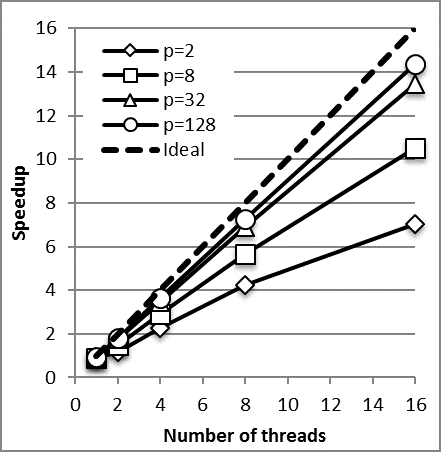
\includegraphics[height=0.28\textheight]{figs/spF2R_2000.png}
	}
	\subfigure[$n = 4000$]{
		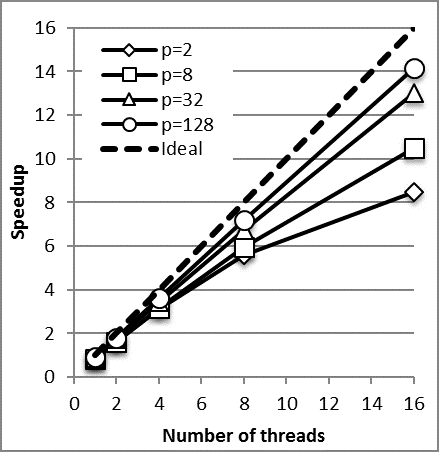
\includegraphics[height=0.28\textheight]{figs/spF2R_4000.png}
	}
	\subfigure[$n = 8000$]{
		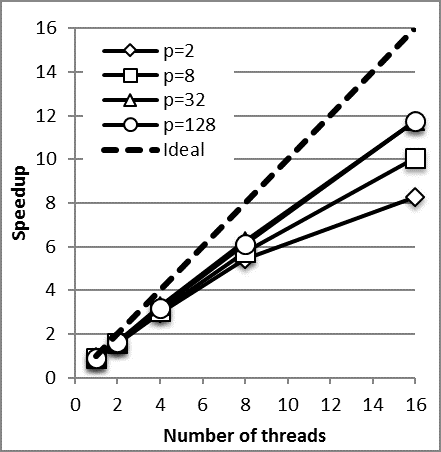
\includegraphics[height=0.28\textheight]{figs/spF2R_8000.png}
	}
	\caption{Speedups obtained with parallel F2R over the sequential PMF construction baseline.}
	\label{fig:f2r-speedup}
\end{figure}

For $p$ values smaller than $128$, i.e., $2$, $8$, and $32$, the average speedups are $7.9$, $10.4$,  and $12.7$, respectively, with $16$ threads. The impact of the parallelization overhead is more for such cases since the amount of the local-queue overhead is proportional to the number of states but not to the number of edges. Consequently, when $p$ decreases the amount of total work decreases and hence, the impact of the overhead increases. Furthermore, since the number of iterations for PMF construction increases with decreasing $p$, the local queues are merged more for smaller $p$ values. Therefore, one can expect more overhead, and hence, less efficiency for smaller $p$ values as the experiments confirm.

\setlength{\tabcolsep}{3pt}
\begin{table}[ht]
	\centering
	\begin{spacing}{1.2}
		\scalebox{0.75}{
			\begin{tabular}{rr|rrrr|rrrr|rrrr}
				\multicolumn{1}{c}{} & \multicolumn{1}{c|}{} & \multicolumn{4}{c|}{n=2000} & \multicolumn{4}{c|}{n=4000} & \multicolumn{4}{c}{n=8000} \\
		
				\multicolumn{1}{c}{} & \multicolumn{1}{c|}{p} & \multicolumn{1}{c}{2} & 		\multicolumn{1}{c}{8} & \multicolumn{1}{c}{32} & \multicolumn{1}{c|}{128} & \multicolumn{1}{c}{2} & \multicolumn{1}{c}{8} & \multicolumn{1}{c}{32} & \multicolumn{1}{c|}{128} & \multicolumn{1}{c}{2} & \multicolumn{1}{c}{8} & \multicolumn{1}{c}{32} & \multicolumn{1}{c}{128} \\ \hline
		 
		 		& sequential & 0.17 & 0.50 & 2.11 & 9.13 & 1.18 & 2.71 & 9.92 & 40.36 & 5.90 & 14.29 & 51.78 & 193.55 \\ \hline
		
			\multirow{3}{*}{1} & F2R & 0.19 & 0.56 & 2.31 & 9.89 & 1.35 & 3.21 & 11.24 & 44.57 & 6.43 & 16.01 & 56.71 & 219.46 \\
		 
		 		& R2F & 0.59 & 0.46 & \textbf{0.85} & 1.91 & 3.17 & 2.61 & 4.72 & 11.39 & 19.41 & 18.17 & 34.35 & 86.60 \\

		 		& Hybrid & \textbf{0.14} & \textbf{0.18} & 0.96 & \textbf{0.65} & \textbf{1.06} & \textbf{0.89} & \textbf{2.99} & \textbf{1.92} & \textbf{5.16} & \textbf{8.42} & \textbf{8.93} & \textbf{5.80} \\ \hline

				\multirow{3}{*}{2} & F2R & 0.15 & 0.34 & 1.21 & 5.00 & 0.73 & 1.68 & 5.74 & 22.41 & 3.82 & 9.14 & 31.40 & 120.23 \\

				& R2F & 0.37 & 0.27 & \textbf{0.46} & 0.98 & 2.00 & 1.55 & 2.62 & 6.04 & 13.73 & 11.96 & 21.54 & 52.67 \\

			& Hybrid & \textbf{0.12} & \textbf{0.14} & 0.53 & \textbf{0.37} & \textbf{0.58} & \textbf{0.50} & \textbf{1.57} & \textbf{1.01} & \textbf{3.09} & \textbf{4.86} & \textbf{5.10} & \textbf{3.34} \\ \hline

				\multirow{3}{*}{4} & F2R & 0.08 & 0.17 & 0.61 & 2.50 & 0.38 & 0.86 & 2.88 & 11.11 & 1.99 & 4.67 & 15.79 & 60.42 \\

				& R2F & 0.20 & 0.15 & \textbf{0.24} & 0.50 & 1.09 & 0.82 & 1.36 & 3.05 & 7.43 & 6.43 & 11.34 & 27.21 \\

				& Hybrid & \textbf{0.06} & \textbf{0.07} & 0.27 & \textbf{0.19} & \textbf{0.31} & \textbf{0.26} & \textbf{0.80} & \textbf{0.52} & \textbf{1.62} & \textbf{2.49} & \textbf{2.61} & \textbf{1.73} \\ \hline

				\multirow{3}{*}{8} & F2R & 0.04 & 0.09 & 0.31 & 1.26 & 0.21 & 0.46 & 1.47 & 5.60 & 1.09 & 2.49 & 8.31 & 31.55 \\

				& R2F & 0.11 & 0.08 & 0.12 & 0.25 & 0.64 & 0.45 & 0.71 & 1.55 & 4.36 & 3.68 & 6.36 & 14.91 \\

				& Hybrid & \textbf{0.03} & \textbf{0.04} & \textbf{0.14} & \textbf{0.10} & \textbf{0.17} & \textbf{0.15} & \textbf{0.42} & \textbf{0.28} & \textbf{0.89} & \textbf{1.34} & \textbf{1.39} & \textbf{0.93} \\ \hline

				\multirow{3}{*}{16} & F2R & \textbf{0.02} & 0.05 & 0.16 & 0.64 & 0.14 & 0.26 & 0.76 & 2.85 & 0.71 & 1.42 & 4.41 & 16.50 \\

				& R2F & 0.06 & 0.04 & 0.06 & 0.13 & 0.41 & 0.26 & 0.38 & 0.81 & 2.78 & 2.38 & 4.06 & 9.10 \\

				& Hybrid & \textbf{0.02} & \textbf{0.02} & \textbf{0.07} & \textbf{0.05} & \textbf{0.12} & \textbf{0.09} & \textbf{0.23} & \textbf{0.16} & \textbf{0.59} & \textbf{0.80} & \textbf{0.80} & \textbf{0.57} \\ \hline

				\multirow{3}{*}{CUDA} & S2R & \textbf{0.02} & \textbf{0.02} & 0.05 & 0.17 & \textbf{0.07} & 0.09 & 0.20 & 0.77 & \textbf{0.31} & 0.39 & 0.92 & 3.36 \\

				& S2F & 0.03 & 0.04 & 0.11 & 0.46 & 0.14 & 0.19 & 0.61 & 2.54 & 0.65 & 0.91 & 4.04 & 13.29 \\

				& Hybrid & \textbf{0.02} & \textbf{0.02} & \textbf{0.03} & \textbf{0.05} & 0.09 & \textbf{0.07} & \textbf{0.12} & \textbf{0.14} & 0.41 & \textbf{0.39} & \textbf{0.46} & \textbf{0.48} \\ \hline

				\multirow{3}{*}{CUDA M.O.} & S2R & \textbf{0.01} & 0.02 & 0.04 & 0.16 & \textbf{0.05} & 0.07 & 0.19 & 0.76 & \textbf{0.21} & 0.31 & 0.85 & 3.33 \\
		
				& S2F & 0.02 & 0.02 & 0.06 & 0.19 & 0.08 & 0.10 & 0.29 & 1.16 & 0.34 & 0.49 & 1.74 & 6.36 \\
		
				& Hybrid & \textbf{0.01} & \textbf{0.01} & \textbf{0.03} & \textbf{0.04} & 0.06 & \textbf{0.05} & \textbf{0.10} & \textbf{0.13} & 0.24 & \textbf{0.28} & \textbf{0.36} & \textbf{0.39}
			\end{tabular}
		}
	\end{spacing}
	\caption{Comparison of the parallel execution times~(in seconds) of the PMF construction algorithms.}
	\label{table:PMF_time}
\end{table}
\setlength{\tabcolsep}{6pt}


Table~\ref{table:PMF_time} compares the execution times of F2R, R2F, S2R, S2F and Hybrid algorithm for $n \in {2000, 4000, 8000}$, $p \in \{2, 8, 32, 128\}$ and $\{1, 2, 4, 8, 16\}$ threads. An interesting observation is that F2R is consistently faster than R2F for $p = 2$, however, it is slower otherwise. This can be explained by the difference in the number of required iterations to construct PMF: when $p$ is large, the frontier expands very quickly and the PMF is constructed in less iterations, e.g., for $n = 2000$, the PMF is generated in $16$ iterations for $p = 2$, whereas only $7$ iterations are required for $p = 8$. Since each edge will be processed once, the runtime of F2R always increases with $p$, i.e., with the number of edges. However, since the frontier expands much faster, the total number of remaining~(R-)pairs processed by the R2F throughout the process will probably decrease. Furthermore, since the frontier is large, while traversing the edge list of an R-pair, it is more probable to early terminate the traversal and add the R-pair to the next frontier earlier. Surprisingly,  when $p$ increases, these may yield a decrease in the R2F runtime~(observe the change from $p = 2$ to $p = 8$ in Table~\ref{table:PMF_time}). However, once the performance benefits of early termination are fully exploited, an increase on the R2F runtime with increasing $p$ is more probable since the overall BFS work, i.e., the total number of edges, also increases with $p$~(observe the change from $p = 8$ to $p = 32$ in Table~\ref{table:PMF_time}).

Observing such performance differences for R2F and F2R on automata with different characteristics, the potential benefit of a Hybrid algorithm in practice is more clear. As Table~\ref{table:PMF_time} shows, the hybrid approach, which is just a combination of F2R and R2F, is almost always faster than employing a pure F2R or a pure R2F BFS-level expansion. Furthermore, we do not need parallelism to observe these performance benefits: the Hybrid approach works better even when a single thread is used at runtime\footnote{Although one can implement F2R, R2F, and Hybrid sequentially, we do not have their sequential variants. With their OpenMP-based implementations, we expect $10\%$ parallelization overhead for both R2F and Hybrid as in F2R since the parallelization techniques employed in the implementations  are similar.}. For example, when $n = 8000$ and $p = 128$, the Hybrid algorithm is $38$ and $15$ times faster than F2R and R2F, respectively. For the same automaton set, the average speedups due to hybridization are $29$ and $16$ with $16$ threads.


\begin{figure}[ht]
	\centering
	\subfigure[$p = 2$]{
		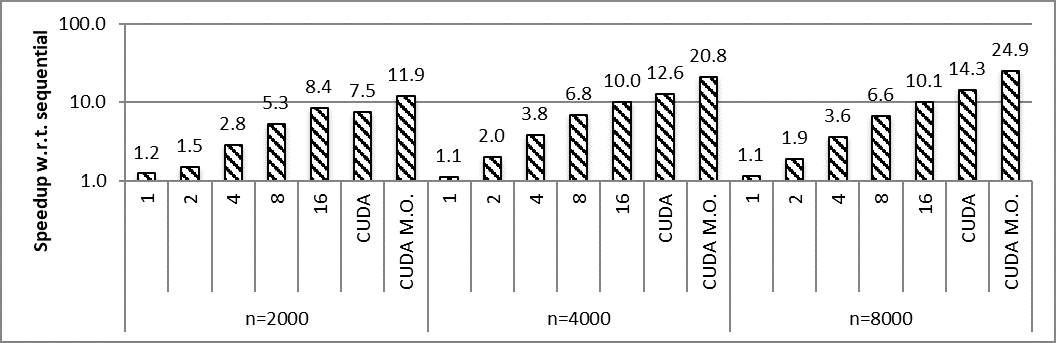
\includegraphics[height=0.17\textheight]{figs/hybrid_speedup_p2.png}
	}
	\subfigure[$p = 8$]{
		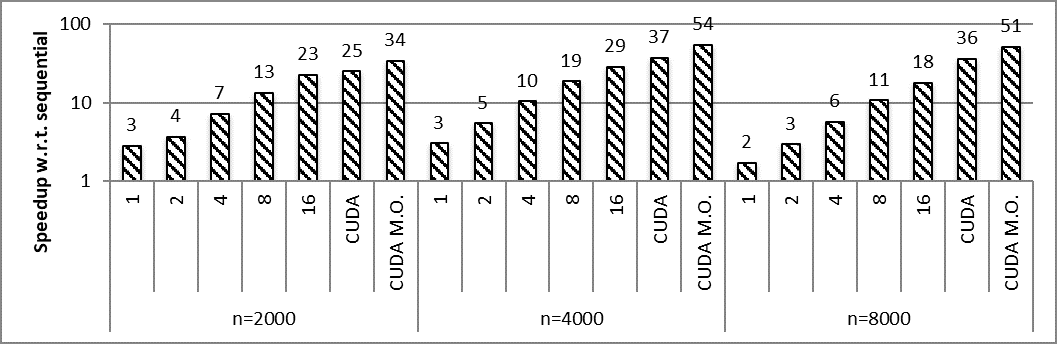
\includegraphics[height=0.17\textheight]{figs/hybrid_speedup_p8.png}
	}
	\subfigure[$p = 32$]{
		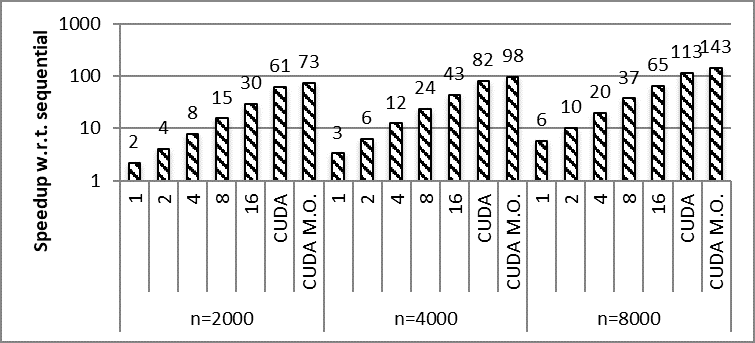
\includegraphics[height=0.17\textheight]{figs/hybrid_speedup_p32.png}
	}	
	\subfigure[$p = 128$]{
		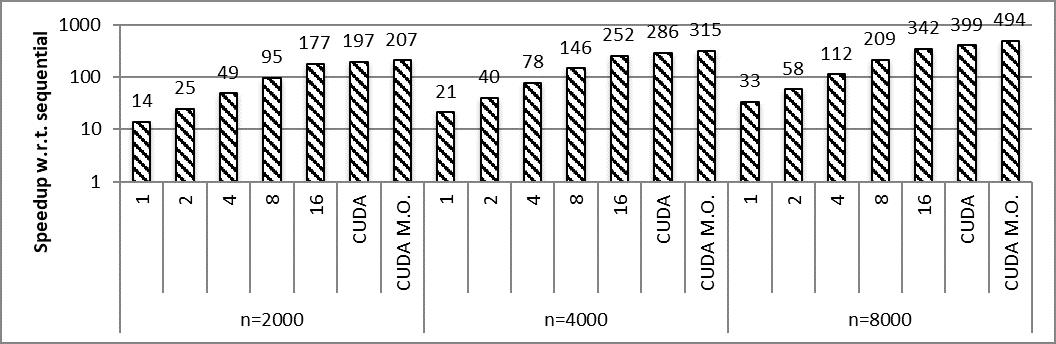
\includegraphics[height=0.17\textheight]{figs/hybrid_speedup_p128.png}
	}
	\caption{The speedups of the Hybrid PMF construction algorithms with ${p=2}$(a), $8$(b), $32$(c), $128$(d) and $n \in \{2000, 4000, 8000\}$. The $x$-axis shows the number of threads used for the Hybrid execution.  The values are computed based on the average sequential PMF construction time over $100$ different automata for each $(n, p)$ pair.}
	\label{fig:hybrid-speedup}
\end{figure}

When the Hybrid algorithm is used, the speedups on the PMF generation phase are given in Figure~\ref{fig:hybrid-speedup}. As the figure shows, thanks to parallelism and good scaling of Hybrid~(for large $p$ values), the speedups increase when the number of threads increases. With the CUDA implementation, the PMF generation process becomes even much faster: the memory optimized version obtains $25$, $51$, $143$, and $494$ speedup for $2$, $8$, $32$, and $128$ letter automata, respectively, with $n = 8000$ states. 

\pagebreak

Since we generate the PMF to find a synchronizing sequence, a more realistic evaluation metric would be the performance improvement over the whole sequential reset sequence construction process. As Table~\ref{table:phase-comparison} shows, for Eppstein's \greedyAlgo\ heuristic~(also for some other heuristics such as \textsc{Cycle}~\cite{Trahtman04}), the PMF generation phase dominates the overall runtime. For this reason, we simply conducted an experiment where the Hybrid approach is used to construct the PMF and no further parallelization is applied during the synchronizing sequence construction phase. Table~\ref{table:phase-comparison-after} shows the speedups for this experiment for all parallel implementations of Hybrid executions. As the results show, when we compared sequential F2R implementation and hybrid implementation with single thread, more than $2$x and more than $14$x improvement is possible for $p = 32$ and $p = 128$, respectively.%\kkcomm{bunu anlamadim, aciklayabilir miyiz? bu 2 ve 14 nereden geldi?} \comment{sertac}{sequential olan yerine tek thread hybrid kullanilinca aldigimiz speeduplar}

\begin{table}[ht]
	\center
	\begin{tabular}{r|rrrr||rrrr}
		& \multicolumn{4}{c||}{Speedup} & \multicolumn{4}{c}{$\frac{t_{PMF}}{t_{ALL}}$}\\ 
		n\textbackslash p  & \multicolumn{1}{c}{2} & \multicolumn{1}{c}{8} & \multicolumn{1}{c}{32} & \multicolumn{1}{c||}{128} & \multicolumn{1}{c}{2} & \multicolumn{1}{c}{8} & \multicolumn{1}{c}{32} & \multicolumn{1}{c}{128} \\ \hline
		2000 & 11.90 & 34.20 & 72.99 & 206.84 & 0.52 & 0.53 & 0.69 & 0.77 \\
		4000 & 20.84 & 54.27 & 97.60 & 315.45 & 0.50 & 0.46 & 0.62 & 0.68 \\
		8000 & 24.92 & 51.00 & 143.01 & 493.97 & 0.36 & 0.39 & 0.45 & 0.47 
	\end{tabular}
	\caption{The speedups obtained on \greedyAlgo\ when the memory optimized CUDA implementation of Hybrid PMF construction algorithm is used.}
	\label{table:phase-comparison-after}
\end{table}

As noted before, F2R-based PMF construction has $O(pn^2)$ time complexity. The R2F-based variant, on the other hand, has $O(dpn^2)$ time complexity (where $d$ is the diameter of the pair automaton ${\cal A}$) since the states of ${\cal A}$ in the remaining set $R$ will be processed at most $d$ times. In practice, however, R2F-based construction (and Hybrid computation which also has $O(dpn^2)$ time complexity since it performs R2F steps) can beat F2R based construction.

We did not perform an extensive study on larger automata since it takes too long with the sequential baseline implementation. For example, sequential PMF generation takes around 2 hours and 30 minutes for an automaton with 40,000 states and 128 letters, whereas our Hybrid implementation generates a sequence in 2 minutes and 30 seconds.

\section{Second Phase Parallelization}

As mentioned in Section \ref{sec:second-phase-parallelization}, the execution time of second phase is worthy to take into account for the slowly synchronizing automata. Hence, we used \v{C}ern\'y automata with $n \in \{ 2000, 4000, 8000 \}$ for completeness of the experiments. For CPU parallelization of second phase, we implemented Algorithm \ref{algo:find-min-parallel} and tested with 1, 2, 4, 8 and 16 threads. For GPU parallelization, we implemented the same algorithm with 256 threads per block and 256 blocks. We also implemented the approach that sorts the set of current active states before the process as mentioned in Section \ref{sec:implementation}.

\begin{table}[ht]
	\center
	\begin{tabular}{rr|rrr}
		& n & 2000 & 4000 & 8000\\\hline
		\multirow{2}{*}{sequential} & unsorted & 4.729 & 41.034 & 1035.093\\
		& sorted & 1.604 & 12.701 & 109.758\\\hline
		\multirow{2}{*}{1} & unsorted & 5.098 & 47.021 & 896.384\\
		& sorted & 2.553 & 20.274 & 168.116\\\hline
		\multirow{2}{*}{2} & unsorted & 3.869 & 37.352 & 874.253\\
		& sorted & 1.935 & 15.085 & 132.770\\\hline
		\multirow{2}{*}{4} & unsorted & 2.308 & 22.705 & 522.930\\
		& sorted & 1.178 & 8.946 & 75.673\\\hline
		\multirow{2}{*}{8} & unsorted & 1.259 & 13.131 & 289.750\\
		& sorted & 0.719 & 5.044 & 40.842\\\hline
		\multirow{2}{*}{16} & unsorted & 0.694 & 6.674 & 154.796\\
		& sorted & 0.723 & 3.350 & 22.403\\\hline
		\multirow{2}{*}{CUDA} & unsorted & 0.684 & 5.514 & 51.280\\
		& sorted & 0.391 & 1.556 & 9.613
	\end{tabular}
	\caption{The execution times~(in seconds) of  Algorithms \ref{algo:find-min} and \ref{algo:find-min-parallel}.}
	\label{table:phase-2-time}
\end{table}

Table \ref{table:phase-2-time} shows that sorting the set of current pairs has a remarkable impact on the performance. Even in sequential implementation, we observed $3\times$ to $9.5\times$ speedups. When both the implementation improvement and GPU parallelization is applied, we observed between $12\times$ and $107\times$ speedups over naive and sequential implementation of the second phase. 

\pagebreak

\section{Speeding up the Fastest}

We call the implementation of \greedyAlgo\ below as the naive baseline implementation. We also implemented the improvements over naive baseline as suggested in Section~\ref{sec:lazy}, Section~\ref{sec:lookahead}, and Section~\ref{sec:smart}. Below, we call these implementations as ``Lazy'', ``Lookahead'', and ``Smart'', respectively. Note that Lookahead is implemented on top of Lazy, and Smart is implemented on top of Lazy and Lookahead.


Figure~\ref{fig:speedups} presents the speedups of each improvement~(i.e. Lazy,  Lookahead, and Smart) over the naive baseline for \greedyAlgo . Lazy computation provides a stable improvement, which is more sensitive to alphabet size $p$. For a given alphabet size, we observe a somewhat constant speed up values. However, the average speedup values increase with the alphabet size. The lookahead also provides a stable improvement and it is more effective. For small alphabet sizes, the speedup provided by the lookahead is almost constant for different number of states. For larger alphabet sizes, on the other hand, the speedup provided by the lookahead increases with the number of states. The effect of the lookahead also increases with the alphabet size. The smart intersection check similarly improves the performance, but not to the same extent as lazy and lookahead.


\begin{figure}[ht]
	\centering
	\subfigure[$p = 2$]{
		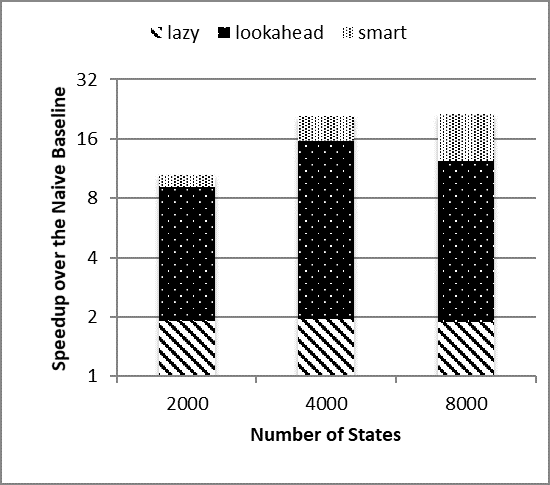
\includegraphics[width=0.47\textwidth]{figs/p2_greedy.png}
	}
	\subfigure[$p = 8$]{
		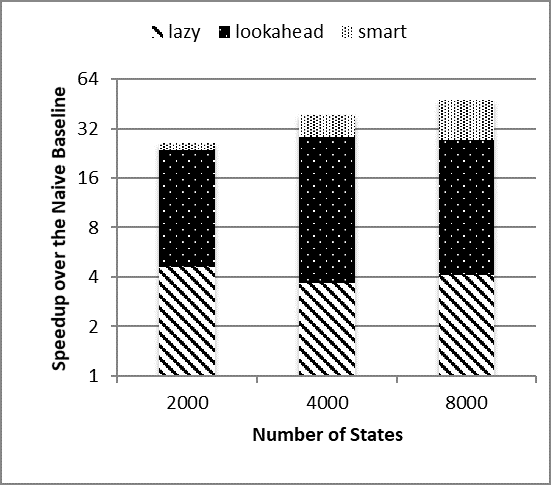
\includegraphics[width=0.47\textwidth]{figs/p8_greedy.png}
	}
	\subfigure[$p = 32$]{
		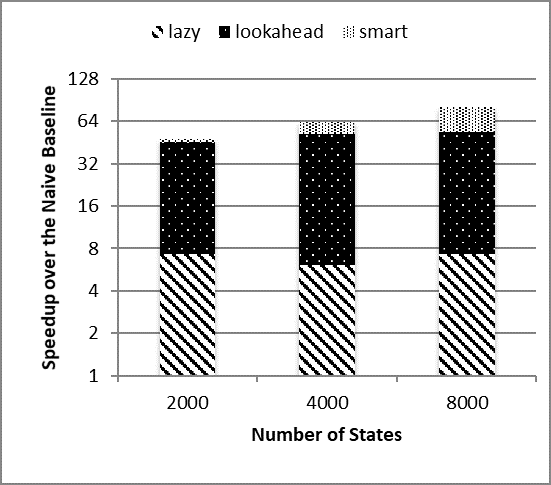
\includegraphics[width=0.47\textwidth]{figs/p32_greedy.png}
	}
	\subfigure[$p = 128$]{
		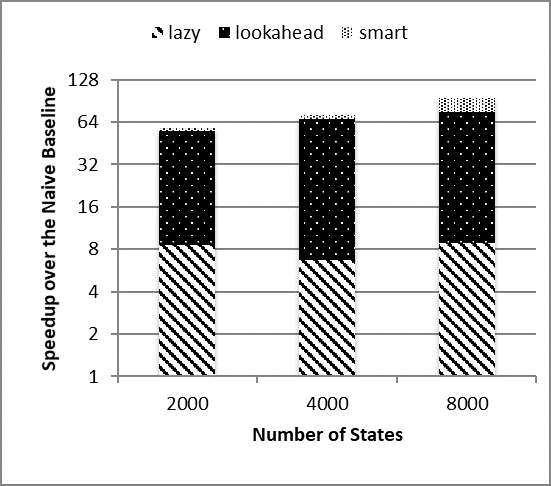
\includegraphics[width=0.47\textwidth]{figs/p128_greedy.png}
	}
	\caption{The speedup values normalized w.r.t. the naive baseline. For each additional improvement, the cumulative speedup is given with stacked columns.}
	\label{fig:speedups}
\end{figure}

Overall, when all the improvements are considered together, the average speedup values shows an increasing trend as the size of the automaton increases, and as we apply more aggressive improvements. We start with $2\times$ speedup for the automata with $n=2000$ and $p=2$ when only the lazy computation is enabled, and we reach to $95\times$ (almost two orders of magnitude) speedup for the automata with $n=8000$ and $p=128$ when all the improvements are enabled.

To validate effectiveness of our methods, we compare the time spent for BFS forest construction in each method. Note that, the time spent in PMF construction is proportional to the number of edges processed. The total number of edges to be processed for an automaton with $n$ states and $p$ letters is $pn(n-1)/2$. Table~\ref{table:edge-percent} reports the percentage of these edges processed by each method.

\begin{table}[ht]
	\center
	\begin{tabular}{rr||r||rrr}
$n$		&	$p$	& Algorithm~\ref{algo:BFS} 	& Lazy		& Lookahaed & Smart \\\hline\hline
2000	& 2		& 99.99\%					& 40.31\%	& 1.71\%	& 1.71\%\\
		& 8		& 84.83\%					& 12.18\%	& 0.56\%	& 0.57\%\\
		& 32	& 37.41\%					& 3.64\%	& 0.25\%	& 0.25\%\\
		& 128	& 11.19\%					& 1.00\%	& 0.11\%	& 0.09\%\\\hline
4000	& 2		& 99.99\%					& 36.92\%	& 1.42\%	& 1.52\%\\
		& 8		& 87.11\%					& 11.72\%	& 0.42\%	& 0.45\%\\
		& 32	& 40.12\%					& 2.93\%	& 0.16\%	& 0.17\%\\
		& 128	& 12.08\%					& 0.94\%	& 0.07\%	& 0.08\%\\\hline
8000	& 2		& 100.00\%					& 37.56\%	& 1.31\%	& 1.24\%\\
		& 8		& 89.16\%					& 12.09\%	& 0.38\%	& 0.33\%\\
		& 32	& 42.78\%					& 3.08\%	& 0.11\%	& 0.06\%\\
		& 128	& 13.02\%					& 0.83\%	& 0.06\%	& 0.05\%
	\end{tabular}
	\caption{The percentage of processed edges}
	\label{table:edge-percent}
\end{table}
First of all, note that even Algorithm~\ref{algo:BFS} does not process all edges. This is caused by the termination condition of the while--loop at line 5. In Algorithm~\ref{algo:BFS}, another possible termination is given at line 5 as a comment: ``$F$ is not empty''. When this alternative termination condition is used, Algorithm~\ref{algo:BFS} processes 100\% of the edges. 

\pagebreak

Recall that the initial motivation for this work is based on the observation that PMF construction time being too high compared to the overall running time of \greedyAlgo . We aimed at reducing this high cost, by modifying \greedyAlgo\ so that they can run without full PMF construction. The figures in Table~\ref{table:edge-percent} show that we succeed. Only a very small part of the PMF is constructed in the modified version of \greedyAlgo\ Algorithm. As the size of the automata increases, the percentage of the PMF constructed decreases.
